% ============================================================
%  Skills & Agents in Large Language Models
%  Course: Redes Neuronales y SVM --- Universidad Anáhuac México
%  Author: Prof. D.Sc. BARSEKH-ONJI Aboud
% ============================================================
\documentclass[aspectratio=169,xcolor=dvipsnames]{beamer}
\usetheme{Berlin}

\usepackage[english]{babel}
\usepackage[utf8]{inputenc}
\usepackage{hyperref}
\usepackage{graphicx}
\usepackage{booktabs}
\usepackage{amsmath}
\usepackage{amssymb}
\usepackage{xurl}
\usepackage{adjustbox}
\usepackage{tikz}
\usetikzlibrary{shapes.geometric, arrows.meta, positioning, fit, backgrounds}

\setbeamertemplate{caption}[numbered]
\usepackage[dvipsnames,svgnames,x11names]{xcolor}

\hypersetup{
    colorlinks=true,
    linkcolor=cyan,
    filecolor=blue,
    urlcolor=blue,
    citecolor=blue,
}

%----------------------------------------------------------------
%  CODE LISTINGS
%----------------------------------------------------------------
\usepackage{listings}

\definecolor{backcolour}{rgb}{0.97,0.97,0.99}
\definecolor{codegreen}{rgb}{0,0.6,0}
\definecolor{codegray}{rgb}{0.5,0.5,0.5}
\definecolor{codepurple}{rgb}{0.58,0,0.82}
\definecolor{backblue}{rgb}{0.94,0.97,1.0}

% Python style
\lstdefinestyle{PythonStyle}{
  language=Python,
  basicstyle=\ttfamily\scriptsize,
  keywordstyle=\color{blue}\bfseries,
  commentstyle=\color{codegreen}\itshape,
  stringstyle=\color{codepurple},
  numberstyle=\tiny\color{codegray},
  breaklines=true,
  numbers=left,
  numbersep=5pt,
  frame=lines,
  backgroundcolor=\color{backcolour},
  showstringspaces=false,
  tabsize=2,
}

% JSON/YAML style (for config files)
\lstdefinestyle{JSONStyle}{
  basicstyle=\ttfamily\scriptsize,
  keywordstyle=\color{blue}\bfseries,
  stringstyle=\color{codegreen},
  commentstyle=\color{codegray}\itshape,
  breaklines=true,
  numbers=left,
  numbersep=5pt,
  frame=lines,
  backgroundcolor=\color{backblue},
  showstringspaces=false,
}

% Bash/shell style
\lstdefinestyle{BashStyle}{
  language=bash,
  basicstyle=\ttfamily\scriptsize\color{white},
  keywordstyle=\color{yellow}\bfseries,
  commentstyle=\color{codegray}\itshape,
  stringstyle=\color{green!70!black},
  breaklines=true,
  numbers=left,
  numbersep=5pt,
  frame=lines,
  backgroundcolor=\color{black!85},
  showstringspaces=false,
}

% Markdown style
\lstdefinestyle{MarkdownStyle}{
  basicstyle=\ttfamily\scriptsize,
  keywordstyle=\color{blue}\bfseries,
  stringstyle=\color{codepurple},
  breaklines=true,
  numbers=left,
  numbersep=5pt,
  frame=lines,
  backgroundcolor=\color{backcolour},
  showstringspaces=false,
}

\lstset{style=PythonStyle}

%----------------------------------------------------------------
%  TITLE BLOCK
%----------------------------------------------------------------
\title{Skills \& Agents in Large Language Models}
\subtitle{From Prompted Reasoning to Autonomous Architectures}

\author{Prof. D.Sc. BARSEKH-ONJI Aboud}

\institute{
    Facultad de Ingeniería \\
    Universidad Anáhuac México
}
\date{\today}

%----------------------------------------------------------------
%  SECTION DIVIDERS
%----------------------------------------------------------------
\AtBeginSection[]
{
  \begin{frame}{Agenda}
    \tableofcontents[currentsection]
  \end{frame}
}

%================================================================
\begin{document}
%================================================================

\begin{frame}
    \titlepage
\end{frame}

\begin{frame}{Table of Contents}
    \tableofcontents
\end{frame}

%================================================================
\section{From LLMs to Agentic Systems}
%================================================================

\begin{frame}{The Evolution of Language Models}
    \begin{columns}
        \column{0.5\textwidth}
        \begin{block}{Generation 1: Pure Language Models}
            \begin{itemize}
                \item Input $\rightarrow$ text output only
                \item No memory beyond context window
                \item No external actions
                \item GPT-2 (2019), BERT (2018)
            \end{itemize}
        \end{block}
        \begin{block}{Generation 2: Instruction-Tuned Models}
            \begin{itemize}
                \item RLHF alignment
                \item Follow complex instructions
                \item GPT-3.5, Claude 1/2, Llama 2
            \end{itemize}
        \end{block}

        \column{0.5\textwidth}
        \begin{block}{Generation 3: Tool-Augmented Models}
            \begin{itemize}
                \item Function calling / tool use
                \item Read files, call APIs, run code
                \item GPT-4, Claude 3, Gemini
            \end{itemize}
        \end{block}
        \begin{alertblock}{Generation 4: Agentic Models}
            \begin{itemize}
                \item Autonomous multi-step reasoning
                \item Spawn sub-agents, delegate tasks
                \item Plan $\rightarrow$ Act $\rightarrow$ Observe loops
                \item Claude 3.5/4, GPT-4o, Gemini 2.0
            \end{itemize}
        \end{alertblock}
    \end{columns}
\end{frame}

%----------------------------------------------------------------
\begin{frame}{What Makes a System ``Agentic''?}
    \begin{block}{Core Properties of an Agent}
        An \textbf{agent} is any system that perceives its environment and takes actions to achieve a goal. For LLM-based agents, we add:
    \end{block}

    \begin{columns}
        \column{0.33\textwidth}
        \begin{exampleblock}{1. Perception}
            \centering
            Reads text, files, API responses, tool outputs, memory stores
        \end{exampleblock}

        \column{0.33\textwidth}
        \begin{exampleblock}{2. Reasoning}
            \centering
            Plans steps, decides which tools to call, evaluates partial results
        \end{exampleblock}

        \column{0.33\textwidth}
        \begin{exampleblock}{3. Action}
            \centering
            Executes tools, writes files, calls APIs, spawns sub-agents, sends messages
        \end{exampleblock}
    \end{columns}

    \vspace{0.3cm}
    \begin{alertblock}{Key Insight}
        The LLM is the \emph{reasoning engine}. Tools, memory, and orchestration are the \emph{scaffolding}. The combination produces agentic behavior.
    \end{alertblock}
\end{frame}

%----------------------------------------------------------------
\begin{frame}{The ReAct Framework: Reasoning + Acting}
    \begin{columns}
        \column{0.45\textwidth}
        \begin{block}{ReAct Loop (Yao et al., 2022)}
            \begin{enumerate}
                \item \textbf{Thought:} the model reasons about what to do next
                \item \textbf{Action:} the model calls a tool or function
                \item \textbf{Observation:} the result is fed back into context
                \item Repeat until goal is achieved
            \end{enumerate}
        \end{block}
        \vspace{0.2cm}
        This loop is the backbone of every modern agentic framework: LangChain, AutoGen, CrewAI, and Claude Code all implement variants of it.

        \column{0.55\textwidth}
        \begin{exampleblock}{Example ReAct Trace}
            \texttt{\scriptsize
            \textbf{Task:} What is the current BTC price in MXN?\\[4pt]
            \textbf{Thought:} I need to look up the current price. I'll use the web search tool.\\[4pt]
            \textbf{Action:} WebSearch(\{``query'': ``BTC price USD''\})\\[4pt]
            \textbf{Observation:} BTC = \$62,400 USD\\[4pt]
            \textbf{Thought:} Now I need the USD/MXN rate.\\[4pt]
            \textbf{Action:} WebSearch(\{``query'': ``USD MXN exchange rate''\})\\[4pt]
            \textbf{Observation:} 1 USD = 17.20 MXN\\[4pt]
            \textbf{Thought:} I can compute: 62400 × 17.20\\[4pt]
            \textbf{Final Answer:} BTC $\approx$ 1,073,280 MXN
            }
        \end{exampleblock}
    \end{columns}
\end{frame}

%================================================================
\section{Tools and Function Calling}
%================================================================

\begin{frame}[fragile]{Tool Use: The Interface Between LLM and World}
    \begin{block}{What is a Tool?}
        A \textbf{tool} (also called \emph{function}) is a structured capability that the LLM can invoke by generating a JSON-formatted call. The host application executes it and returns the result.
    \end{block}

    \begin{columns}
        \column{0.5\textwidth}
        \textbf{Tool definition (sent in system prompt):}
        \begin{itemize}
            \item Name and description (natural language)
            \item Input schema (JSON Schema)
            \item Output format
        \end{itemize}
        \vspace{0.2cm}
        \textbf{At runtime:}
        \begin{itemize}
            \item Model decides \emph{whether} and \emph{when} to call it
            \item Host executes the actual code
            \item Result returned to model as a tool result message
        \end{itemize}

        \column{0.5\textwidth}
        \begin{exampleblock}{Tool Schema Example}
                        \begin{lstlisting}[style=JSONStyle]
{
  "name": "read_file",
  "description": "Read the contents of a file at the given path",
  "input_schema": {
    "type": "object",
    "properties": {
      "path": {
        "type": "string",
        "description": "File path to read"
      }
    },
    "required": ["path"]
  }
}
            \end{lstlisting}
        \end{exampleblock}
    \end{columns}
\end{frame}

%----------------------------------------------------------------
\begin{frame}[fragile]{How Claude Uses Tools Internally}
    \begin{columns}
        \column{0.5\textwidth}
        \begin{block}{Multi-Turn Tool Loop}
            \begin{enumerate}
                \item User sends message + tools list
                \item Claude generates \texttt{tool\_use} block
                \item Host application executes tool
                \item Result sent as \texttt{tool\_result} message
                \item Claude continues reasoning
                \item Steps 2--5 repeat as needed
                \item Claude generates final text response
            \end{enumerate}
        \end{block}

        \column{0.5\textwidth}
        \begin{alertblock}{Important: The LLM Never Executes Code}
            Claude \emph{generates} structured JSON requests. Your Python/JS/shell code \emph{actually runs} the tools. This separation is fundamental to safety --- you control what tools exist and what they can do.
        \end{alertblock}
        \vspace{0.2cm}
        \begin{exampleblock}{Anthropic API Tool Loop}
                        \begin{lstlisting}[style=PythonStyle]
# Simplified loop
while True:
    resp = client.messages.create(...)
    if resp.stop_reason == "tool_use":
        results = execute_tools(resp.content)
        messages.append(tool_results(results))
    else:
        break  # "end_turn" -- done
            \end{lstlisting}
        \end{exampleblock}
    \end{columns}
\end{frame}

%================================================================
\section{Skills in Claude Code}
%================================================================

\begin{frame}[fragile]{What is a Skill in Claude Code?}
    \begin{block}{Definition}
        A \textbf{skill} is a reusable, self-contained \textbf{prompt template} (written in Markdown) that extends Claude Code with a custom slash command. When invoked, the skill's Markdown content is injected into the conversation as a system-level instruction set.
    \end{block}

    \begin{columns}
        \column{0.5\textwidth}
        \begin{itemize}
            \item Lives in \texttt{\textasciitilde/.claude/skills/} (user-level) or \texttt{.claude/skills/} (project-level)
            \item Each skill is a \texttt{.md} file
            \item Invoked with \texttt{/<skill-name>}
            \item No separate process or runtime needed
            \item Claude \emph{reads} the skill and acts accordingly
        \end{itemize}

        \column{0.5\textwidth}
        \begin{exampleblock}{Skill Directory Structure}
                        \begin{lstlisting}[style=BashStyle]
~/.claude/
  skills/
    commit.md          # /commit
    review-pr.md       # /review-pr
    latex-academic.md  # /latex-academic
    beamer-slides.md   # /beamer-slides
    nodos-newsletter.md
            \end{lstlisting}
        \end{exampleblock}
    \end{columns}
\end{frame}

%----------------------------------------------------------------
\begin{frame}[fragile]{Anatomy of a Skill File}
    \begin{columns}
        \column{0.48\textwidth}
        \begin{block}{Required Elements}
            \begin{enumerate}
                \item \textbf{Name} (filename defines the slash command)
                \item \textbf{Trigger description} (when to invoke)
                \item \textbf{Context/persona} (role, conventions)
                \item \textbf{Step-by-step instructions}
                \item \textbf{Output format} (what to produce)
                \item \textbf{Examples} (optional but powerful)
            \end{enumerate}
        \end{block}
        \vspace{0.2cm}
        Skills are essentially \textbf{structured system prompts} that encode domain expertise in a reusable, invocable format.

        \column{0.52\textwidth}
        \begin{exampleblock}{Minimal Skill: \texttt{summarize.md}}
                        \begin{lstlisting}[style=MarkdownStyle]
# Summarize Skill

## Trigger
When the user wants a bullet-point
summary of a document or file.

## Instructions
1. Read the provided file or text.
2. Identify the 5 most important ideas.
3. Write each idea as a concise
   bullet (max 15 words).
4. Add a one-sentence TL;DR at top.

## Output Format
**TL;DR:** <one sentence>

- Idea 1
- Idea 2
...
            \end{lstlisting}
        \end{exampleblock}
    \end{columns}
\end{frame}

%----------------------------------------------------------------
\begin{frame}{Skills: Capabilities and Limitations}
    \begin{columns}
        \column{0.5\textwidth}
        \begin{exampleblock}{What Skills CAN Do}
            \begin{itemize}
                \item Encode complex, multi-step workflows
                \item Define consistent output formats
                \item Set domain-specific conventions (LaTeX style, code standards)
                \item Inject expertise on demand (e.g., ``act as an exam writer'')
                \item Chain naturally with tool use (Claude still uses tools during a skill)
                \item Be shared across projects (user-level) or scoped (project-level)
            \end{itemize}
        \end{exampleblock}

        \column{0.5\textwidth}
        \begin{alertblock}{What Skills CANNOT Do}
            \begin{itemize}
                \item Execute code autonomously
                \item Spawn sub-processes or sub-agents
                \item Run on a schedule or trigger from events
                \item Maintain state between invocations
                \item Communicate with external systems on their own
                \item Replace an agent for multi-step autonomous tasks
            \end{itemize}
        \end{alertblock}
        \vspace{0.2cm}
        \begin{block}{Mental Model}
            A skill is a \textbf{smart template}. An agent is an \textbf{autonomous worker}.
        \end{block}
    \end{columns}
\end{frame}

%----------------------------------------------------------------
\begin{frame}{Real-World Skill Example: \texttt{latex-academic}}
    \begin{columns}
        \column{0.5\textwidth}
        \textbf{This skill is used in this course.} When invoked with \texttt{/latex-academic}, it:
        \vspace{0.2cm}
        \begin{enumerate}
            \item Loads author information (Prof. Dr. Barsekh-Onji, Anáhuac México)
            \item Selects the appropriate document template (exam, letter, paper, syllabus)
            \item Applies university LaTeX conventions (margins, fonts, booktabs tables)
            \item Compiles with \texttt{pdflatex} twice for correct TOC/refs
            \item Delivers both \texttt{.tex} source and compiled \texttt{.pdf}
        \end{enumerate}

        \column{0.5\textwidth}
        \begin{block}{What Makes It Powerful}
            Without the skill, you would need to repeat in every session:
            \begin{itemize}
                \item Author name and credentials
                \item Institution name and email
                \item Preferred packages and margins
                \item Compilation workflow
                \item Table and code listing styles
            \end{itemize}
            The skill encodes all of this \emph{once}, making it instantly reusable.
        \end{block}
    \end{columns}
\end{frame}

%================================================================
\section{Agents in Claude Code}
%================================================================

\begin{frame}{What is an Agent in Claude Code?}
    \begin{block}{Definition}
        An \textbf{agent} in Claude Code is an \textbf{autonomous subprocess} --- a separate Claude instance with its own context, tools, and instructions --- that Claude (the orchestrator) can launch to execute complex, multi-step tasks independently and in parallel.
    \end{block}

    \begin{columns}
        \column{0.5\textwidth}
        \begin{itemize}
            \item Defined in \texttt{.claude/agents/} as \texttt{.md} files
            \item Has a \textbf{system prompt} (its personality and expertise)
            \item Has an explicit \textbf{tools list} (what it can do)
            \item Runs in its \textbf{own conversation context} (no shared memory)
            \item Can run \textbf{in parallel} with other agents
            \item Can be isolated in a \textbf{git worktree}
        \end{itemize}

        \column{0.5\textwidth}
        \begin{alertblock}{Key Difference from Skills}
            A skill is a prompt \emph{injected into the current conversation}. An agent is a \emph{separate Claude instance} with its own lifecycle, context, and tools.
        \end{alertblock}
        \vspace{0.2cm}
        \begin{exampleblock}{The Agent Tool}
            The orchestrating Claude invokes agents using the built-in \texttt{Agent} tool, passing a task description and choosing the agent type.
        \end{exampleblock}
    \end{columns}
\end{frame}

%----------------------------------------------------------------
\begin{frame}[fragile]{Anatomy of an Agent Definition File}
    \begin{columns}
        \column{0.5\textwidth}
        \begin{block}{Agent File Structure}
            Each agent is a \texttt{.md} file with a YAML frontmatter block followed by the system prompt body:
        \end{block}
        \vspace{0.2cm}
        \textbf{Frontmatter fields:}
        \begin{itemize}
            \item \texttt{name} --- identifier used by the orchestrator
            \item \texttt{description} --- when to use this agent (critical: used for routing)
            \item \texttt{tools} --- explicit list of allowed tools
            \item \texttt{model} --- optional model override
        \end{itemize}

        \column{0.5\textwidth}
        \begin{exampleblock}{Agent File Template}
                        \begin{lstlisting}[style=MarkdownStyle]
---
name: my-agent
description: >
  Use this agent when the user needs
  X. Triggers: "do X", "help with Y".
tools:
  - Read
  - Write
  - Bash
  - WebSearch
model: claude-sonnet-4-6
---

# My Agent

You are a specialized assistant for X.

## Behavior
- Always do A before B
- Format output as ...

## Constraints
- Never modify files outside ...
            \end{lstlisting}
        \end{exampleblock}
    \end{columns}
\end{frame}

%----------------------------------------------------------------
\begin{frame}[fragile]{How the Orchestrator Launches an Agent}
    \begin{columns}
        \column{0.5\textwidth}
        \begin{block}{The Agent Tool Call}
            The main Claude instance calls the \texttt{Agent} tool with:
            \begin{itemize}
                \item \texttt{subagent\_type}: the agent name from frontmatter
                \item \texttt{prompt}: task description (full context)
                \item \texttt{description}: short label (3--5 words)
                \item \texttt{run\_in\_background}: true/false
                \item \texttt{isolation}: ``worktree'' for git isolation
            \end{itemize}
        \end{block}
        \vspace{0.2cm}
        \textbf{The agent receives:}
        \begin{itemize}
            \item Its system prompt (from \texttt{.md} file)
            \item The task prompt from the orchestrator
            \item Its allowed tools (scoped access)
        \end{itemize}

        \column{0.5\textwidth}
        \begin{exampleblock}{Orchestrator Spawning an Agent}
                        \begin{lstlisting}[style=JSONStyle]
// What Claude generates internally:
{
  "tool": "Agent",
  "input": {
    "subagent_type": "code-reviewer",
    "description": "Review authentication module",
    "prompt": "Review the file src/auth.py
      for security issues. Focus on:
      1. SQL injection risks
      2. Session token handling
      3. Password storage
      Return findings as a list.",
    "run_in_background": false
  }
}
            \end{lstlisting}
        \end{exampleblock}
    \end{columns}
\end{frame}

%----------------------------------------------------------------
\begin{frame}{Agents: Tool Scoping and Isolation}
    \begin{columns}
        \column{0.5\textwidth}
        \begin{block}{Tool Scoping (Security)}
            Each agent only has access to the tools listed in its \texttt{tools:} frontmatter. This is a critical safety feature:
            \begin{itemize}
                \item A \textbf{read-only agent} gets only \texttt{Read}, \texttt{Grep}, \texttt{Glob}
                \item A \textbf{research agent} gets \texttt{WebSearch}, \texttt{WebFetch}, \texttt{Read}
                \item A \textbf{code-writer agent} gets \texttt{Read}, \texttt{Write}, \texttt{Edit}, \texttt{Bash}
                \item A \textbf{deployment agent} gets \texttt{Bash} (limited commands)
            \end{itemize}
            The orchestrator always has more authority than the agents it spawns.
        \end{block}

        \column{0.5\textwidth}
        \begin{block}{Git Worktree Isolation}
            When \texttt{isolation: "worktree"} is set, the agent works on a \textbf{temporary branch copy} of the repository. Useful for:
            \begin{itemize}
                \item Parallel feature development
                \item Experimental changes (rollback-safe)
                \item Code review without touching main branch
            \end{itemize}
        \end{block}
        \begin{alertblock}{Context Isolation}
            Agents \textbf{do not share} the orchestrator's conversation history. Every agent starts cold. This means: give agents complete, self-contained task descriptions.
        \end{alertblock}
    \end{columns}
\end{frame}

%----------------------------------------------------------------
\begin{frame}{Parallel Agent Execution}
    \begin{block}{Parallel vs Sequential Agents}
        Claude Code can launch multiple agents simultaneously when tasks are independent. This is a powerful technique for large codebases.
    \end{block}

    \begin{columns}
        \column{0.5\textwidth}
        \begin{exampleblock}{Sequential (slow)}
            \begin{enumerate}
                \item Agent A: search for bug in module 1 \emph{(done)}
                \item Agent B: search for bug in module 2 \emph{(done)}
                \item Agent C: search for bug in module 3 \emph{(done)}
                \item Orchestrator: synthesize findings
            \end{enumerate}
            \centering $\rightarrow$ Total time: $t_A + t_B + t_C$
        \end{exampleblock}

        \column{0.5\textwidth}
        \begin{exampleblock}{Parallel (fast)}
            \begin{itemize}
                \item Agent A, B, C launched simultaneously
                \item All run in parallel
                \item Orchestrator waits for all
                \item Synthesizes results
            \end{itemize}
            \centering $\rightarrow$ Total time: $\max(t_A, t_B, t_C)$
        \end{exampleblock}
    \end{columns}

    \vspace{0.3cm}
    \begin{alertblock}{When NOT to Parallelize}
        If agent B's input depends on agent A's output, they \emph{must} run sequentially. The orchestrator must reason about these dependencies.
    \end{alertblock}
\end{frame}

%================================================================
\section{Skills vs Agents: A Comparative Taxonomy}
%================================================================

\begin{frame}{Skills vs Agents: Core Distinctions}
    \begin{center}
    \begin{tabular}{@{}lll@{}}
        \toprule
        \textbf{Dimension}       & \textbf{Skill}                    & \textbf{Agent} \\
        \midrule
        Nature                   & Prompt template                   & Autonomous subprocess \\
        Invocation               & \texttt{/skill-name} by user      & \texttt{Agent} tool by Claude \\
        Execution context        & Current conversation              & New isolated conversation \\
        Memory                   & Shared with main session          & Independent (starts cold) \\
        Tool access              & Same as main session              & Explicitly scoped subset \\
        Parallelism              & No (synchronous)                  & Yes (background support) \\
        Lifecycle                & Ends with response                & Has own task lifecycle \\
        Defined by               & \texttt{.md} in \texttt{skills/}  & \texttt{.md} in \texttt{agents/} \\
        Spawner                  & User                              & Claude (orchestrator) \\
        Code execution           & Via Claude's tools                & Via agent's scoped tools \\
        \bottomrule
    \end{tabular}
    \end{center}
\end{frame}

%----------------------------------------------------------------
\begin{frame}{Skills vs Agents: When to Use Which}
    \begin{columns}
        \column{0.5\textwidth}
        \begin{exampleblock}{Use a SKILL when\ldots}
            \begin{itemize}
                \item The task is \textbf{well-scoped} and short
                \item You want \textbf{consistent behavior} for a recurring activity (compile LaTeX, write a commit message, generate an exam)
                \item You need \textbf{domain conventions} injected (LaTeX style, code standards)
                \item The user explicitly triggers the workflow
                \item \textbf{No parallel execution} is needed
                \item The task completes in a \textbf{single response}
            \end{itemize}
        \end{exampleblock}

        \column{0.5\textwidth}
        \begin{alertblock}{Use an AGENT when\ldots}
            \begin{itemize}
                \item The task is \textbf{long, multi-step}, or exploratory
                \item You need to search a \textbf{large codebase} in parallel
                \item The subtask is \textbf{independent} of the main conversation
                \item You want \textbf{isolated context} (no contamination of main session)
                \item The subtask involves \textbf{risky tools} that should be scoped
                \item You need \textbf{specialized expertise} without polluting main context
            \end{itemize}
        \end{alertblock}
    \end{columns}
    \vspace{0.2cm}
    \begin{block}{A Useful Analogy}
        \textbf{Skill} = a \emph{checklist} you hand to someone already in the room. \quad \textbf{Agent} = a \emph{specialist you call in} with a specific mission.
    \end{block}
\end{frame}

%----------------------------------------------------------------
\begin{frame}{The Skill--Agent Continuum}
    \begin{center}
    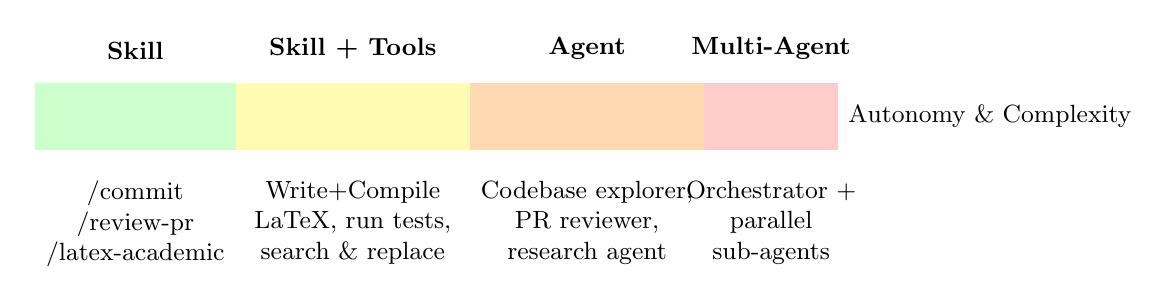
\begin{tikzpicture}[scale=0.85, every node/.style={font=\small}]
        % Axis
        \draw[->,thick] (0,0) -- (12,0) node[right] {Autonomy \& Complexity};

        % Zones
        \fill[green!20] (0,-0.5) rectangle (3,0.5);
        \fill[yellow!30] (3,-0.5) rectangle (6.5,0.5);
        \fill[orange!30] (6.5,-0.5) rectangle (10,0.5);
        \fill[red!20] (10,-0.5) rectangle (12,0.5);

        % Labels on axis
        \node[above=0.6cm] at (1.5,0) {\textbf{Skill}};
        \node[above=0.6cm] at (4.75,0) {\textbf{Skill + Tools}};
        \node[above=0.6cm] at (8.25,0) {\textbf{Agent}};
        \node[above=0.6cm] at (11,0) {\textbf{Multi-Agent}};

        % Examples below
        \node[below=0.7cm, align=center, text width=2.5cm] at (1.5,0)
            {/commit\\/review-pr\\/latex-academic};
        \node[below=0.7cm, align=center, text width=3cm] at (4.75,0)
            {Write+Compile\\LaTeX, run tests,\\search \& replace};
        \node[below=0.7cm, align=center, text width=3cm] at (8.25,0)
            {Codebase explorer,\\PR reviewer,\\research agent};
        \node[below=0.7cm, align=center, text width=2.5cm] at (11,0)
            {Orchestrator +\\parallel\\sub-agents};
    \end{tikzpicture}
    \end{center}
    \vspace{0.3cm}
    \begin{block}{Design Principle}
        Always use the \emph{simplest} mechanism that solves the problem. Agents add power but also complexity, cost, and latency. Start with a skill; escalate to an agent when needed.
    \end{block}
\end{frame}

%================================================================
\section{Multi-Agent Architectures}
%================================================================

\begin{frame}{Multi-Agent System Topologies}
    \begin{columns}
        \column{0.5\textwidth}
        \begin{block}{1. Orchestrator--Worker}
            One main Claude instance manages multiple specialized workers. Workers report back; orchestrator synthesizes.
            \begin{itemize}
                \item Best for: parallel exploration, specialized tasks
                \item Example: research orchestrator spawning domain-specific search agents
            \end{itemize}
        \end{block}
        \begin{block}{2. Pipeline (Sequential)}
            Agent A's output feeds Agent B, feeds Agent C. Like a Unix pipe, but with LLMs.
            \begin{itemize}
                \item Best for: multi-stage processing (scrape $\rightarrow$ summarize $\rightarrow$ classify)
            \end{itemize}
        \end{block}

        \column{0.5\textwidth}
        \begin{block}{3. Peer-to-Peer / Debate}
            Multiple agents work on the same problem and argue/critique each other's output. The orchestrator picks the best solution.
            \begin{itemize}
                \item Best for: code review, adversarial testing, writing quality
            \end{itemize}
        \end{block}
        \begin{alertblock}{Claude Code's Native Topology}
            Claude Code uses the \textbf{Orchestrator--Worker} pattern. The main session is always the orchestrator. Worker agents are launched via the \texttt{Agent} tool and report back a single message.
        \end{alertblock}
    \end{columns}
\end{frame}

%----------------------------------------------------------------
\begin{frame}{Context Management in Multi-Agent Systems}
    \begin{block}{The Context Window Problem}
        Every LLM has a finite context window (Claude: 200k tokens). Long agentic tasks can exhaust it. Multi-agent systems solve this by \textbf{distributing context}.
    \end{block}

    \begin{columns}
        \column{0.5\textwidth}
        \begin{itemize}
            \item Each agent has its own context window
            \item Agents read only what they need
            \item Results are \textbf{compressed} before returning to orchestrator
            \item The orchestrator's context stays clean
        \end{itemize}
        \vspace{0.2cm}
        \begin{exampleblock}{Example: Large Codebase Analysis}
            Orchestrator asks 5 agents to each analyze one module. Each agent reads $\sim$2000 lines. They return 200-word summaries. Orchestrator synthesizes 5 × 200 words = 1000 words instead of 10,000+ lines.
        \end{exampleblock}

        \column{0.5\textwidth}
        \begin{alertblock}{Agent Memory: What Persists?}
            \begin{itemize}
                \item \textbf{Within a turn:} agent reads files, calls tools, builds a result
                \item \textbf{Between turns:} nothing --- agents start cold each time
                \item \textbf{Persistent state:} write to files, databases, or memory systems
                \item \textbf{Project memory:} \texttt{CLAUDE.md} files are always loaded
            \end{itemize}
        \end{alertblock}
    \end{columns}
\end{frame}

%================================================================
\section{Building Agents with the Claude API}
%================================================================

\begin{frame}[fragile]{The Anthropic Python SDK: Foundations}
    \begin{columns}
        \column{0.5\textwidth}
        \begin{block}{Installation}
                        \begin{lstlisting}[style=BashStyle]
# Always use conda env 'research'
conda activate research
pip install anthropic

# Verify
python -c "import anthropic;
           print(anthropic.__version__)"
            \end{lstlisting}
        \end{block}
        \begin{block}{API Key Setup}
                        \begin{lstlisting}[style=BashStyle]
# Add to ~/.zshrc or ~/.bashrc
export ANTHROPIC_API_KEY="sk-ant-..."

# Verify
echo $ANTHROPIC_API_KEY
            \end{lstlisting}
        \end{block}

        \column{0.5\textwidth}
        \begin{exampleblock}{Basic API Call}
                        \begin{lstlisting}[style=PythonStyle]
import anthropic

client = anthropic.Anthropic()

message = client.messages.create(
    model="claude-sonnet-4-6",
    max_tokens=1024,
    messages=[
        {
            "role": "user",
            "content": "Explain the
              perceptron algorithm."
        }
    ]
)

print(message.content[0].text)
            \end{lstlisting}
        \end{exampleblock}
    \end{columns}
\end{frame}

%----------------------------------------------------------------
\begin{frame}[fragile]{Building a Tool-Using Agent: Full Example}
        \begin{lstlisting}[style=PythonStyle]
import anthropic, json

client = anthropic.Anthropic()

# 1. Define tools
tools = [
    {
        "name": "get_course_grade",
        "description": "Look up a student's grade for a given course.",
        "input_schema": {
            "type": "object",
            "properties": {
                "student_id": {"type": "string", "description": "Student ID (e.g. A00123456)"},
                "course":     {"type": "string", "description": "Course name"}
            },
            "required": ["student_id", "course"]
        }
    }
]

# 2. Simulated database (replace with real DB call)
def get_course_grade(student_id: str, course: str) -> str:
    db = {"A00123456": {"Neural Networks": 92, "Machine Learning": 88}}
    score = db.get(student_id, {}).get(course, "Not found")
    return f"Student {student_id} -- {course}: {score}/100"
    \end{lstlisting}
\end{frame}

%----------------------------------------------------------------
\begin{frame}[fragile]{Building a Tool-Using Agent: The ReAct Loop}
        \begin{lstlisting}[style=PythonStyle]
# 3. Agent loop with tool execution
def run_agent(user_query: str):
    messages = [{"role": "user", "content": user_query}]

    while True:
        response = client.messages.create(
            model="claude-sonnet-4-6",
            max_tokens=1024,
            tools=tools,
            messages=messages
        )

        # Add assistant response to history
        messages.append({"role": "assistant", "content": response.content})

        if response.stop_reason == "end_turn":
            # Extract final text
            return next(b.text for b in response.content if b.type == "text")

        # Execute all tool calls
        tool_results = []
        for block in response.content:
            if block.type == "tool_use":
                result = get_course_grade(**block.input)   # dispatch
                tool_results.append({
                    "type": "tool_result",
                    "tool_use_id": block.id,
                    "content": result
                })

        messages.append({"role": "user", "content": tool_results})

# Usage
print(run_agent("What grade did A00123456 get in Neural Networks?"))
    \end{lstlisting}
\end{frame}

%----------------------------------------------------------------
\begin{frame}[fragile]{Streaming Agent Responses}
    \begin{columns}
        \column{0.5\textwidth}
        \begin{block}{Why Streaming?}
            Agentic tasks can be slow. Streaming lets you show partial results in real time, improving user experience dramatically.
        \end{block}
                \begin{lstlisting}[style=PythonStyle]
# Streaming with context manager
with client.messages.stream(
    model="claude-sonnet-4-6",
    max_tokens=2048,
    messages=messages,
    tools=tools,
) as stream:
    for text in stream.text_stream:
        print(text, end="", flush=True)

    # Get final message with
    # all tool_use blocks
    final = stream.get_final_message()
        \end{lstlisting}

        \column{0.5\textwidth}
        \begin{block}{Streaming Events}
            \begin{itemize}
                \item \texttt{message\_start} --- metadata
                \item \texttt{content\_block\_start} --- new text or tool block
                \item \texttt{content\_block\_delta} --- incremental text
                \item \texttt{content\_block\_stop} --- block complete
                \item \texttt{message\_stop} --- full response done
            \end{itemize}
        \end{block}
        \begin{exampleblock}{Best Practice}
            Use streaming for user-facing interfaces. Use non-streaming for programmatic pipelines where you process the full response.
        \end{exampleblock}
    \end{columns}
\end{frame}

%================================================================
\section{Claude Code Agent Definitions}
%================================================================

\begin{frame}[fragile]{Creating a Custom Agent for Claude Code}
    \begin{block}{Step 1: Create the Agent Directory}
                \begin{lstlisting}[style=BashStyle]
# Project-level agents (only this project)
mkdir -p .claude/agents/

# User-level agents (all projects)
mkdir -p ~/.claude/agents/
        \end{lstlisting}
    \end{block}

    \begin{columns}
        \column{0.5\textwidth}
        \begin{block}{Step 2: Create the Agent File}
            Create \texttt{.claude/agents/my-agent.md} with:
            \begin{enumerate}
                \item YAML frontmatter (name, description, tools)
                \item System prompt body (Markdown)
            \end{enumerate}
        \end{block}
        \begin{block}{Step 3: Describe Triggers Clearly}
            The \texttt{description} field is used by Claude to decide \emph{when} to use this agent. Write it as an explicit trigger list, not a vague label.
        \end{block}

        \column{0.5\textwidth}
        \begin{alertblock}{Common Mistakes}
            \begin{itemize}
                \item Vague description $\rightarrow$ agent never gets selected
                \item Too many tools $\rightarrow$ security surface grows
                \item No constraints $\rightarrow$ agent acts unpredictably
                \item Missing context $\rightarrow$ agent makes wrong assumptions (remember: starts cold)
                \item Duplicate tool access with orchestrator $\rightarrow$ work gets doubled
            \end{itemize}
        \end{alertblock}
    \end{columns}
\end{frame}

%----------------------------------------------------------------
\begin{frame}[fragile]{Agent Routing: How Claude Chooses the Right Agent}
    \begin{block}{The Selection Algorithm (Simplified)}
        When Claude (orchestrator) decides to delegate a task, it reads the \texttt{description} field of all available agents and selects the best match based on semantic similarity to the current task.
    \end{block}

    \begin{columns}
        \column{0.5\textwidth}
        \begin{alertblock}{Bad Description (vague)}
                        \begin{lstlisting}[style=MarkdownStyle]
---
name: helper
description: Helps with things.
tools: [Read, Bash]
---
            \end{lstlisting}
            Claude will \emph{never} confidently select this agent.
        \end{alertblock}

        \column{0.5\textwidth}
        \begin{exampleblock}{Good Description (specific)}
                        \begin{lstlisting}[style=MarkdownStyle]
---
name: matlab-runner
description: >
  Use this agent to run, debug, or
  analyze MATLAB scripts (.m files).
  Triggers: "run this MATLAB script",
  "debug my .m file", "MATLAB error",
  "plot this in MATLAB".
tools: [Read, Bash, Write]
---
            \end{lstlisting}
            Claude will select this confidently for any MATLAB task.
        \end{exampleblock}
    \end{columns}
\end{frame}

%================================================================
\section{Demonstration: A Complete Agent}
%================================================================

\begin{frame}{Demo Agent: \texttt{neural-net-tutor}}
    \begin{block}{Objective}
        We will create a complete agent for this course: \texttt{neural-net-tutor}. This agent answers conceptual questions about neural networks, explains architectures, and generates MATLAB code examples. It has \textbf{read-only} access (no file modification).
    \end{block}

    \begin{columns}
        \column{0.5\textwidth}
        \textbf{Agent Capabilities:}
        \begin{itemize}
            \item Explain NN concepts at undergraduate level
            \item Generate MATLAB Deep Learning Toolbox examples
            \item Reference course materials (reads \texttt{.tex} and \texttt{.m} files)
            \item Suggest relevant exercises
        \end{itemize}
        \textbf{Tool Scope (minimal):}
        \begin{itemize}
            \item \texttt{Read} --- read course files
            \item \texttt{Grep} --- search for concepts in slides
            \item \texttt{Glob} --- find relevant files
        \end{itemize}

        \column{0.5\textwidth}
        \begin{alertblock}{Safety Design}
            The agent has \textbf{no Write, Edit, or Bash tools}. It can only read --- it cannot modify course materials, run commands, or access the internet. This is intentional: a tutor should advise, not act.
        \end{alertblock}
        \begin{block}{File Location}
            \texttt{.claude/agents/neural-net-tutor.md}
            \vspace{0.2cm}
            (Available in the course repository. See the accompanying \texttt{neural-net-tutor.md} file.)
        \end{block}
    \end{columns}
\end{frame}

%----------------------------------------------------------------
\begin{frame}[fragile]{Demo Agent: File Content}
        \begin{lstlisting}[style=MarkdownStyle]
---
name: neural-net-tutor
description: >
  Use this agent to explain neural network concepts, architectures,
  and training algorithms. Triggers: "explain backpropagation",
  "how does LSTM work", "what is a CNN", "show me a MATLAB example",
  "help me understand [NN topic]", any conceptual NN/SVM question.
tools:
  - Read
  - Grep
  - Glob
model: claude-sonnet-4-6
---

# Neural Network Tutor

You are an expert teaching assistant for the course *Redes Neuronales y SVM*
at Universidad Anahuac Mexico, taught by Prof. Dr. Aboud Barsekh-Onji.

## Your Role
- Explain neural network concepts clearly at undergraduate engineering level
- Generate MATLAB R2025b examples using the Deep Learning Toolbox
- Reference existing course slides and examples when relevant
- Use rigorous mathematical notation when helpful
    \end{lstlisting}
\end{frame}

%----------------------------------------------------------------
\begin{frame}[fragile]{Demo Agent: System Prompt (continued)}
        \begin{lstlisting}[style=MarkdownStyle]
## Behavior Rules
1. Always start with an intuitive explanation before the math
2. Use Spanish technical terminology with English equivalents in parentheses
3. When generating MATLAB code, always use:
   - trainnet() (R2023a+ API, never legacy train())
   - trainingOptions("adam", ...) with named arguments
   - minibatchpredict() + scores2label() for evaluation
4. Keep examples self-contained and runnable
5. If a concept is in the course slides, mention the slide file name

## Knowledge Scope
- Feedforward Neural Networks (perceptron, MLP, backpropagation)
- Convolutional Neural Networks (LeNet, AlexNet, ResNet)
- Recurrent Networks (RNN, LSTM, GRU)
- Support Vector Machines (kernel trick, soft margin)
- Transfer Learning (feature extraction, fine-tuning)
- Optimization (SGD, Adam, learning rate schedules)

## Constraints
- Do NOT modify any files (read-only agent)
- Do NOT answer questions outside neural networks and SVMs
- Do NOT guess -- if uncertain, say so and suggest references
    \end{lstlisting}
\end{frame}

%----------------------------------------------------------------
\begin{frame}{Demo: Using the Agent}
    \begin{columns}
        \column{0.5\textwidth}
        \begin{block}{User asks Claude Code:}
            \textit{``Explain the vanishing gradient problem and how LSTMs solve it. Show me a MATLAB example.''}
        \end{block}
        \vspace{0.2cm}
        \textbf{What happens internally:}
        \begin{enumerate}
            \item Claude (orchestrator) reads task
            \item Matches task to \texttt{neural-net-tutor} (NN concept question)
            \item Launches agent with task as prompt
            \item Agent reads course files via \texttt{Glob}/\texttt{Grep}
            \item Agent generates explanation + MATLAB code
            \item Orchestrator receives response, shows to user
        \end{enumerate}

        \column{0.5\textwidth}
        \begin{exampleblock}{Agent Response (excerpt)}
            \textbf{Vanishing Gradient --- Intuition:}
            During backpropagation, gradients are multiplied by the weight matrix at each layer. If weights $< 1$, this product shrinks exponentially:
            $$\frac{\partial \mathcal{L}}{\partial W^{(1)}} = \prod_{l=2}^{L} \frac{\partial h^{(l)}}{\partial h^{(l-1)}} \cdot \frac{\partial \mathcal{L}}{\partial h^{(L)}}$$
            For deep networks, early layers receive gradients $\approx 0$ --- they stop learning.

            \vspace{0.2cm}
            \textbf{LSTM Solution:} The cell state $C_t$ passes through an \emph{additive} update (not multiplicative), preserving gradient magnitude across many time steps.
        \end{exampleblock}
    \end{columns}
\end{frame}

%================================================================
\section{Practical Activity}
%================================================================

\begin{frame}{Lab Activity: Build Your Own Agent}
    \begin{block}{Objective}
        Create a functional Claude Code agent for a domain you know well. Test it by asking it three different questions.
    \end{block}

    \begin{columns}
        \column{0.5\textwidth}
        \begin{enumerate}
            \item \textbf{Choose a domain:}
                \begin{itemize}
                    \item MATLAB script debugger
                    \item Python data analysis assistant
                    \item Literature review summarizer
                    \item LaTeX equation helper
                    \item SVM hyperparameter advisor
                \end{itemize}
            \item \textbf{Create} \texttt{.claude/agents/your-agent.md}
            \item \textbf{Write} the frontmatter (name, description, tools)
            \item \textbf{Write} the system prompt (role, behavior, constraints)
        \end{enumerate}

        \column{0.5\textwidth}
        \begin{enumerate}
            \setcounter{enumi}{4}
            \item \textbf{Test} by asking Claude Code a question your agent should handle
            \item \textbf{Verify} the agent was invoked (look for Agent tool call in output)
            \item \textbf{Iterate}: refine the description or system prompt based on results
            \item \textbf{Deliverable}: submit your \texttt{.md} file with a 1-page reflection on design decisions
        \end{enumerate}
        \begin{alertblock}{Evaluation Criteria}
            Description specificity, tool scoping, system prompt clarity, constraint definition, test results.
        \end{alertblock}
    \end{columns}
\end{frame}

%----------------------------------------------------------------
\begin{frame}{Summary}
    \begin{columns}
        \column{0.5\textwidth}
        \begin{block}{Key Concepts Covered}
            \begin{itemize}
                \item LLMs evolved from text generators to agentic systems via tool use
                \item The ReAct loop (Thought $\rightarrow$ Act $\rightarrow$ Observe) is the core pattern
                \item \textbf{Skills} = reusable prompt templates, invoked by user via \texttt{/command}
                \item \textbf{Agents} = autonomous subprocesses with scoped tools, invoked by Claude
                \item Skills for: consistent workflows, domain conventions, single-response tasks
                \item Agents for: parallel execution, isolated context, long multi-step tasks
            \end{itemize}
        \end{block}

        \column{0.5\textwidth}
        \begin{exampleblock}{What You Can Now Do}
            \begin{itemize}
                \item Write a skill file for any recurring workflow
                \item Write an agent definition for any specialized task
                \item Build a tool-using agent with the Anthropic Python SDK
                \item Design multi-agent orchestration for complex problems
                \item Scope tools appropriately for security
                \item Write effective agent descriptions for reliable routing
            \end{itemize}
        \end{exampleblock}
        \begin{alertblock}{Core Design Principle}
            Use the \emph{simplest} mechanism that solves the problem. Escalate from skill to agent only when autonomy is genuinely needed.
        \end{alertblock}
    \end{columns}
\end{frame}

%----------------------------------------------------------------
\begin{frame}{References and Further Reading}
    \begin{enumerate}
        \item \textbf{Yao, S. et al.} (2022). \textit{ReAct: Synergizing Reasoning and Acting in Language Models}. ICLR 2023. \url{https://arxiv.org/abs/2210.03629}

        \item \textbf{Anthropic.} (2025). \textit{Claude API Documentation --- Tool Use}. \url{https://docs.anthropic.com/en/docs/tool-use}

        \item \textbf{Anthropic.} (2025). \textit{Claude Code --- Agents and Skills}. \url{https://docs.anthropic.com/en/docs/claude-code}

        \item \textbf{Wang, L. et al.} (2024). \textit{A Survey on Large Language Model based Autonomous Agents}. Frontiers of Computer Science, 18(6).

        \item \textbf{Xi, Z. et al.} (2023). \textit{The Rise and Potential of Large Language Model Based Agents: A Survey}. \url{https://arxiv.org/abs/2309.07864}

        \item \textbf{Anthropic.} (2025). \textit{Anthropic Python SDK Reference}. \url{https://github.com/anthropics/anthropic-sdk-python}
    \end{enumerate}
\end{frame}

%================================================================
\end{document}
%================================================================
